\section{DRAM Technology and Scaling}

DRAM technology has continually advanced through capacitor scaling, high-$k$ dielectrics, and process innovations. 
Maintaining sufficient cell capacitance while suppressing leakage becomes increasingly difficult at deep sub-20\,nm nodes \cite{choi2022}. 
To extend scaling, 3D DRAM concepts---stacking capacitor arrays analogous to 3D NAND---are explored \cite{iedm2023_dram}, 
though integration complexity and refresh overhead remain open challenges \cite{kim2021_dram}.

% ==== Fig.1: Speed (access time) vs. retention (TikZ/PGFPlots) ====
\begin{figure}[!t]
\centering
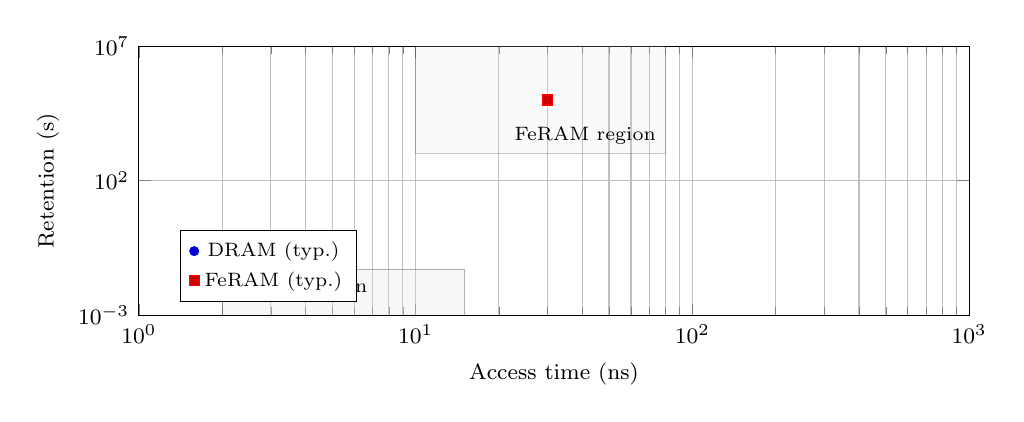
\begin{tikzpicture}
\begin{loglogaxis}[
  width=\linewidth,
  height=5.0cm,
  xlabel={Access time (ns)},
  ylabel={Retention (s)},
  xmin=1e0, xmax=1e3,
  ymin=1e-3, ymax=1e7,
  grid=both,
  legend style={at={(0.05,0.05)},anchor=south west, font=\scriptsize},
  label style={font=\footnotesize},
  tick label style={font=\footnotesize}
]
% Typical points (conceptual)
\addplot+[only marks,mark=*,mark size=1.6pt] coordinates {(5, 1e-2)};     
\addlegendentry{DRAM (typ.)}
\addplot+[only marks,mark=square*,mark size=1.8pt] coordinates {(30, 1e5)}; 
\addlegendentry{FeRAM (typ.)}

% DRAM region (conceptual)
\addplot [draw=black, fill=black!10, opacity=0.3] 
  coordinates {(2,1e-3) (15,1e-3) (15,5e-2) (2,5e-2)} -- cycle;
% FeRAM region (conceptual)
\addplot [draw=black, fill=black!10, opacity=0.2] 
  coordinates {(10,1e3) (80,1e3) (80,1e7) (10,1e7)} -- cycle;

\node[anchor=north west, font=\scriptsize] at (axis cs:2,5e-2) {DRAM region};
\node[anchor=south east, font=\scriptsize] at (axis cs:80,1e3) {FeRAM region};
\end{loglogaxis}
\end{tikzpicture}
\caption{Speed vs.\ retention (conceptual). DRAM is faster but requires refresh; FeRAM offers long retention at modest access times.}
\label{fig:speed_retention}
\end{figure}
